\documentclass{article}

% Symbols
\usepackage{amsfonts, amsthm}
\usepackage{upgreek}
\usepackage{physics}
\usepackage{cancel}
\usepackage{amssymb, latexsym, amsmath}
\usepackage{import}

%Algorithms
\usepackage[ruled,lined,linesnumbered,commentsnumbered]{algorithm2e}

%% Identación
\setlength{\parindent}{0cm}

% Código
\newcommand{\code}[1]{\textcolor{white!25!black}{\texttt{#1}}}
\usepackage{listings}

%AMS
\usepackage{amsthm}
\newtheorem{algo-thm}{Algoritmo}

% Graphics
\usepackage{graphicx}
\usepackage{pgf}

% Margins
\addtolength{\voffset}{-1.5cm}
\addtolength{\hoffset}{-1.5cm}
\addtolength{\textwidth}{3cm}
\addtolength{\textheight}{3cm}

%Header-Footer
\usepackage{fancyhdr}
\renewcommand{\headrulewidth}{1pt}

\newcommand{\set}[1]{
  \left\{ #1 \right\}
}

\footskip = 50pt
\renewcommand{\headrulewidth}{1pt}

\pagestyle{fancyplain}

\begin{document}
\title{UNIVERSIDAD NACIONAL AUT\'ONOMA DE M\'EXICO\\ Facultad de Ciencias}
\author{Integrantes:\\
  Diego Angel Rosas Franco\\
  Adri\'an Aguilera Moreno\\
  Marco Antonio Rivera Silva}
\date{}
\maketitle
\begin{center}
  
\includegraphics[scale=0.20]{../Portada/Portada}\\[0.4cm]
  \Large
  \bf{Modelado y programación}
  \normalsize
\end{center}
\newpage
\fancyhead[r]{ Modelado y programación 2022-2}


\section*{\LARGE{Práctica 4}}

Menciona los principios de diseño esenciales de los patrones Factory, Abstract Factory y Builder.
Menciona una desventaja de cada patrón.

\subsubsection*{Factory}
Principios de diseño:
\newcommand{\localtextbulletone}{\textcolor{black}{\raisebox{.45ex}{\rule{.6ex}{.6ex}}}}
\renewcommand{\labelitemi}{\localtextbulletone}
\begin{itemize}
\item Se define una interfaz para crear objetos, pero permite decidir entre varias subclases cuál se usará para instanciar
\item Se tiene un método conocido conceptualmente como "Factory Method" encargado de la creación de objetos segun las subclases.
\item Encapsula las partes de código que cambian, de las que no cambian en un objeto sin exponer la lógica de creación al cliente.
\item Ayuda que el código no dependa especificamente de alguna clase, lo cual ayuda a modularizar el proyecto.

\end{itemize}
Desventajas:
\begin{itemize}

\item Al extender el sistema, cuando se agrega una nueva clase, se deberá modificar el Factory Method considerando las nuevas clases. 
Esto es una desventaja pues estamos exponiendo el código a modificaciones inesperadas (por ejemplo).
\end{itemize}

\subsubsection*{Abstract Factory}
Principios de diseño:
\begin{itemize}
\item El patrón funciona alrededor de una "fábrica" que crea "fábricas".
\item Una interfaz es responsable de crear una fábrica de objetos relacionados sin especificar explícitamente las clases que involucran dichos objetos.
\item Cada fábrica generada crea objetos como se establece en el patrón Factory. 

\end{itemize}
Desventajas:
\begin{itemize}
\item Cada vez que necesitemos anexar otra entidad, necesitaremos una "Fábrica" extra, es decir, una interfaz que administre los objetos de este tipo de entidad.
\item El sistema crece mucho si se abusa del patrón, y esto lo hace más complejo mediante la creacion de clases para administrar objetos.
\end{itemize}

\subsubsection*{Builder}
Principios de diseño:
\begin{itemize}
	\item Permite construír distintas representaciones de objetos complejos mediante el uso de constructores de objetos simples.
	\item La construcción de estos objetos complejos dependerá de un constructor o director que tratará a cada componente como una etapa de la construcción.
	\item Se pueden tener directores concretos que se dediquen a un objeto complejo especígfico o directores abstractos que permitirán la construcción cualquier combinación de componentes.
	\item Cada componente está modularizado, lo cual nos permite cambiar el orden de construcción con facilidad.
	\item Encapsula la forma en que se construye un objeto complejo.
	\item Permite que los objetos se construyan en un proceso de varios pasos y variable (a diferencia de las fábricas que es un solo paso).
\end{itemize}
Desventajas:
\begin{itemize}
\item La construcción de objetos requiere más conocimiento del dominio del cliente, ya que de no tener claro desde un inicio todas las posibilidades o la estructura final de los objetos, vamos a tener que estar modificando el código constantemente.

\end{itemize}


\subsection*{Instrucciones de instalación, compilación y ejecución.}
Se dará por hecho que el usuario sabe moverse en terminal.\\

\subsubsection*{Requerimientos previos:}
\begin{itemize}
\item[-] Se debe contar con Java en su computadora. De preferencia la versión más reciente.
\end{itemize}

\subsubsection*{Ejecución del proyecto:}
\begin{itemize}
\item[-] Si está leyendo esto significa que desempaquetó con éxito el proyecto.
\item[-] Abra su terminal y diríjase a la ruta donde desempaquetó el proyecto.
\item[-] Una vez estando en la ruta \code{Practica04\_NullPointerException}, diríjase a
  \code{Practica04\_NullPointerException/src/fciencias/modelado/}
\item[-] Ejecute: “\code{javac TallerNaves.java}”, esto generará los .class del proyecto.
\item[-] Ejecute: “\code{java TallerNaves}”, esto ejecutará el proyecto mostrándole el menú solicitado para la practica.
\subsubsection{Lista de Estadisticas de las Partes de la Nave}
\begin{table}[]
	\centering
	\begin{tabular}{|c|c|c|c|c|c|}
		\hline
		Tipo Coponente & Precio & Peso & Ataque & Defensa & Velocidad \\ \hline
		Laser Simple & 79,834.99\$ & 999.52 kg & 7 & 2 & - \\
		Misiles de Plasma & 298,777.99\$ & 1,987.52 kg & 23 & 2 & - \\
		Laser Destructor de Planetas & 945,785.99\$ & 10,000.52 kg & 50 & 2 & - \\
		Blindaje Simple & 50,000.50\$ & 4,900.90 kg & - & 5 & - \\
		Blindaje Reforzado & 145,000.00\$ & 9,975.87 kg & - & 15 & - \\
		Blindaje Fortaleza & 385.000.00\$ & 49750.80 kg & - & 50 & - \\
		Cabina Un Piloto & 19,878.99\$ & 1,986.10 kg & - & 2 & - \\
		Cabina Tripulación Pequeña & 69,876.00\$ & 4,899.52 kg & - & 5 & - \\
		Cabina Ejercito & 199.789.99\$ & 34,567.00 kg & - & 10 & - \\
		Propulsión Viaje Intercontinental & 105,000.00\$ & 997.90 kg & - & 1 & 100 \\
		Propulsión Viaje Interplanetario & 294.000.00\$ & 2,985.90 kg & - & 3 & 500 \\
		Propulsión Viaje Intergalactico & 875,000.00\$ & 9,950.49 kg & - & 5 & 1000 \\ \hline
	\end{tabular}
\end{table}
\end{itemize}

\subsubsection*{Justificación de uso de patrón:}


\newpage
\subsection*{Tabla de Componentes:}


\newpage
\subsection*{Diagrama UML:}
\begin{center}
	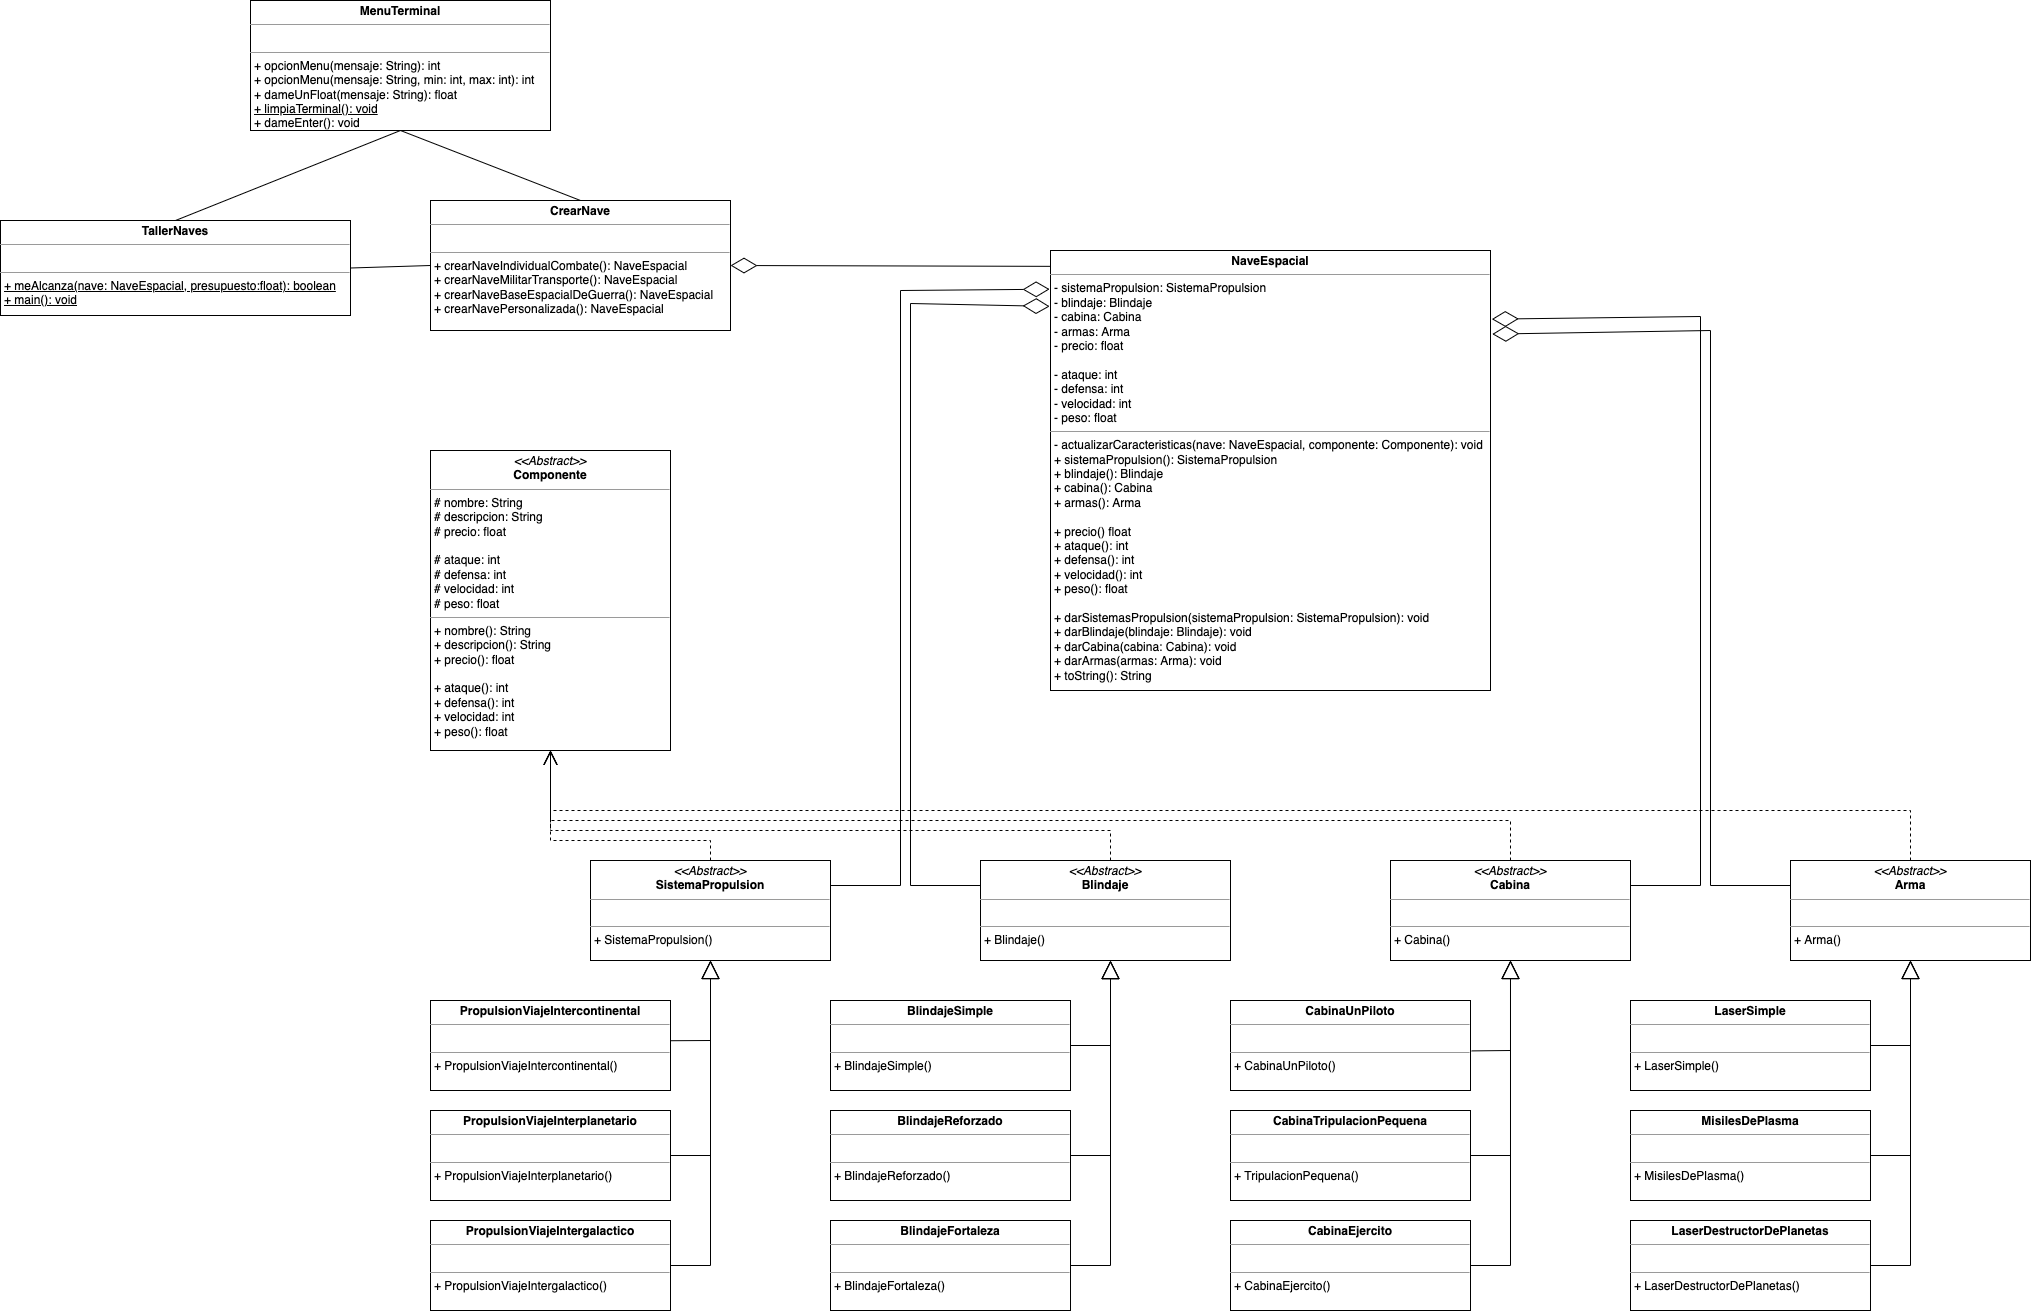
\includegraphics[scale=0.16]{./Practica04UML.png}
\end{center}
\end{document}
